
\newpage
\section{Design}

\subsection*{Existing Systems}
- Current design papers
- Gamification elements

\subsection{Implementing Rewards}
- Vision
  - Send notification
  - Show nice visuals
- Audio
  - Send notification
  - Play uplifting music
- Tactic
  - A.P.I. sets wearable alarm
  - Wearable (fitbit) issues and tracks alarm times

\subsubsection*{Methods of implementation}
- 3 Types:
  1. specific apps
    - Bad cuz takes a long time
  2. Web Apps
    - Still another app
  3. Chatbot
    - Good useful
- Android/iOS/chatbot specific notifications from web app
- Save to home screen

Web app could be chosen because its easiest and achievable, however the ease of use with a chatbot, integrated into fb messenger means everyone can use it on multiple devices. The addition, means that people get used to the UI.

\subsection{Components}
  [app] -------> (Database) -----> at certain time ---> Send notification to trigger type of reward
  [ big button that says track]
  taskname textbox


\subsection{Chatbots}

\subsubsection*{How 2 build and deliver these rewards to users}

\subsubsection*{Current Chatbots}

  - Setup:
    - Setup the bot via a messaging platform, such as fb messenger
  - Trigger:
      - Either A, certain configured time of the day
      -        B: No trigger
      -        C: Around a specific time
  - Action:
    - Choose habit from list of habits
    - Perform
    - Use app to track the action
  - Reward:
    - You get one of these rewards, based on modalitiy selected
    - Vision
      - Through message, of an image or gif
      - Could be: App, or message, gif
    - Audatory
      - Through phone via bot, link to mp3/spotify/apple music
      - Could be: App
    - Tactic
      - Through wearable
      - Could be: App, bot triggers wearbale alarm

FB messenger

\begin{figure}[ht] % ht
    \centering
    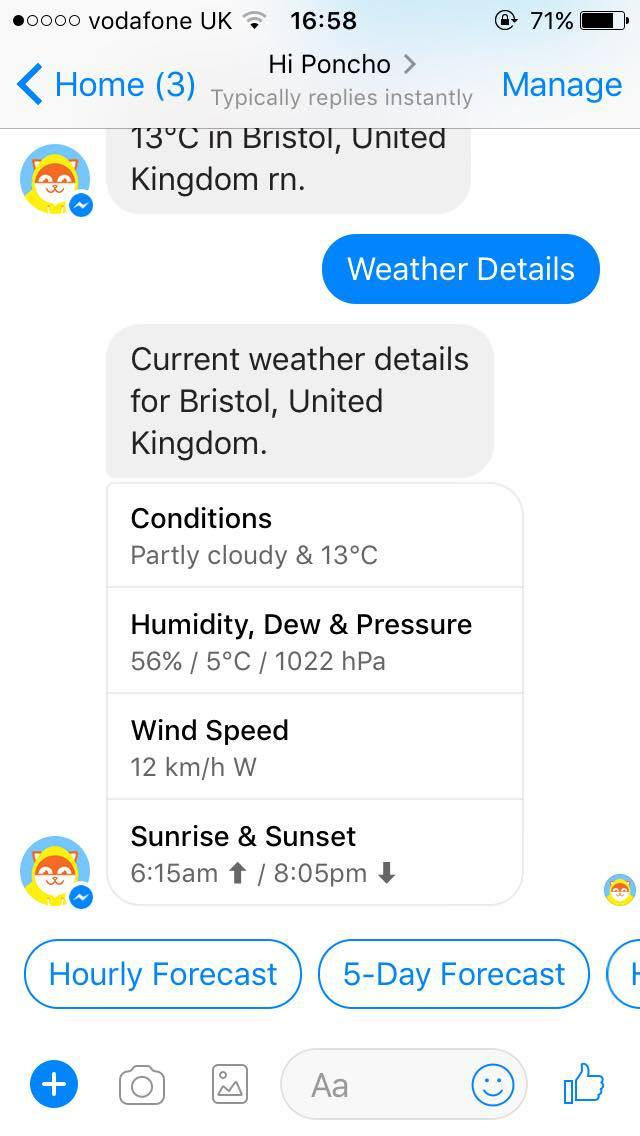
\includegraphics[width=3.2in]{../resources/poncho.jpg}
    \caption{Poncho: A Facebook Messenger Weather Chatbot}
    \label{fig:poncho}
\end{figure}

\subsubsection*{Training a chatbot}

\subsection{Design Requirements}

\subsection{Scope}

@TODO Scope and is the relevance of the reviewed work to the project is always made clear?


\subsection{User Flow}
  - Pre-Start
    - Choose daily habit type from list of X, e.g. 1 press up before breakfast
    - Enable notifications or fitbit if chosen
    - Time action / reward, variable rewards, e.g. then work out average time to send, or none
  - Start:
    - New day
    - @ trigger time, send reminder, if set, notification
    - Open notification, do habit, press tracked
    - Get reward type
